\documentclass[12pt]{article}
\usepackage{amsmath}
\usepackage{amsfonts}
\usepackage{graphicx}
\usepackage[margin=2.5cm]{geometry}

\newcounter{eqn}
\renewcommand*{\theeqn}{A\arabic{eqn})}
\newcommand{\num}{\refstepcounter{eqn}\text{\theeqn}\;}

\makeatletter
\newcommand{\putindeepbox}[2][0.7\baselineskip]{{%
    \setbox0=\hbox{#2}%
    \setbox0=\vbox{\noindent\hsize=\wd0\unhbox0}
    \@tempdima=\dp0
    \advance\@tempdima by \ht0
    \advance\@tempdima by -#1\relax
    \dp0=\@tempdima
    \ht0=#1\relax
    \box0
}}
\makeatother

\begin{document}
\Large

\vspace*{10px}
\begin{center}
\huge{Can't Get No Boolean Satisfaction}
\end{center}
\vspace*{10px}

\vspace{.2in}
You walk into the math lounge and immediately see strange expressions scribbled on the wall. Around the lounge
there are $8$ numbered chess tables. In front of all the tables is written: 

\begin{center}
``Follow where the piece lands. The light is One, the dark is None.''

\underline{\hspace{1cm}} \underline{\hspace{1cm}} \underline{\hspace{1cm}} \underline{\hspace{1cm}} 
\end{center}

\vspace{.2in}

$$\lor = \texttt{ OR, } \land = \texttt{ AND, } \oplus = \texttt{ XOR, } \overline{x} = \texttt{ NOT x}$$


\vspace{.3in}


\[ \begin{array}{ccc}
    1. & a \lor \overline{(b \land c)} \lor d = A1; & \texttt{(A1, ?, 1, 0)} \\
    2. & (a \land b) \land (c \oplus d) = A2; & \texttt{(1, A2, ?, 1)} \\ 
        \\
    3. & \overline{(a \oplus b) \land (c \oplus d)} = A3; & \texttt{(A3, 1, 1, ?)} \\
    4. & (a \lor b) \oplus (\overline{c} \land d) = A4; & \texttt{(0, 0, ?, A4)} \\
        \\
    5. & (a \oplus b) \land (c \lor \overline{d}) = A5; & \texttt{(0, 1, ?, A5)} \\
    6. & (a \lor b \land \overline{c}) \oplus d = A6; & \texttt{(0, A6, ?, 0)} \\
        \\
    7. & (a \lor b) \land (c \oplus \overline{d}) = A7; & \texttt{(A7, 1, ?, 0)} \\
    8. & (a \oplus b \oplus c \oplus d) = A8; & \texttt{(A8, 0, ?, 0)} \\
\end{array} \]

\newpage

\begin{tabular}{cc}
    \num\putindeepbox[7pt]{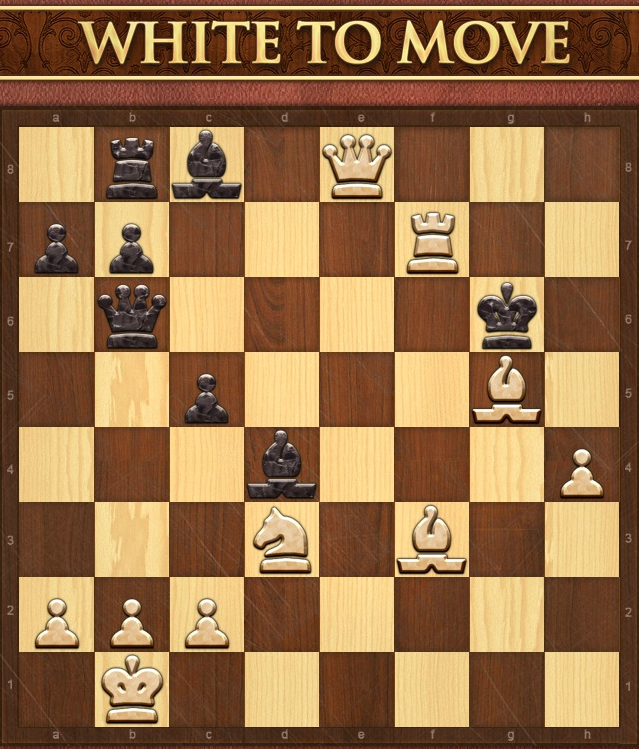
\includegraphics[scale=0.4]{cropped-boards/1-crop.png}}
    & \num\putindeepbox[7pt]{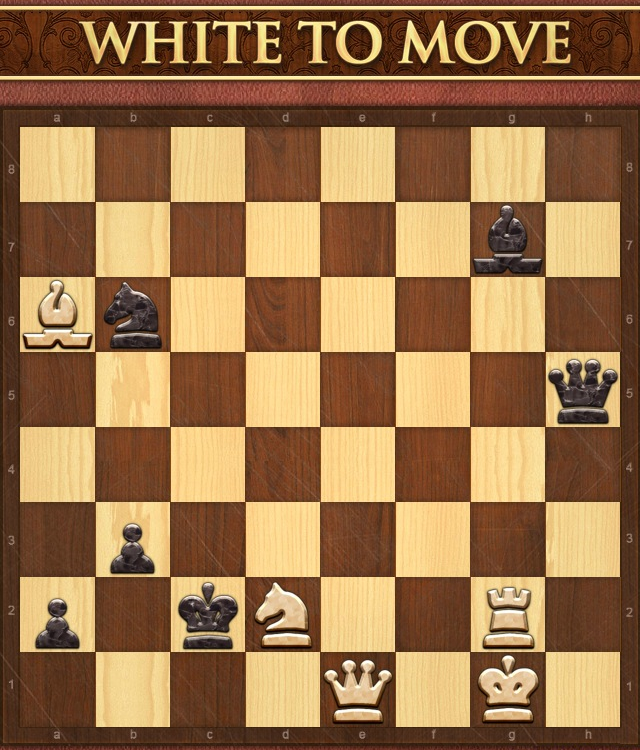
\includegraphics[scale=0.4]{cropped-boards/2-crop.png}} \\
    \num\putindeepbox[7pt]{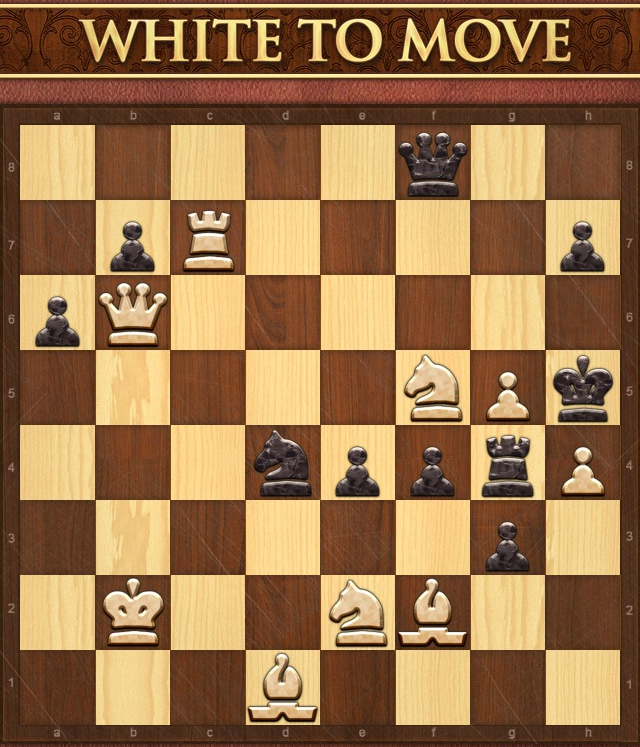
\includegraphics[scale=0.4]{cropped-boards/3-crop.png}}
    & \num\putindeepbox[7pt]{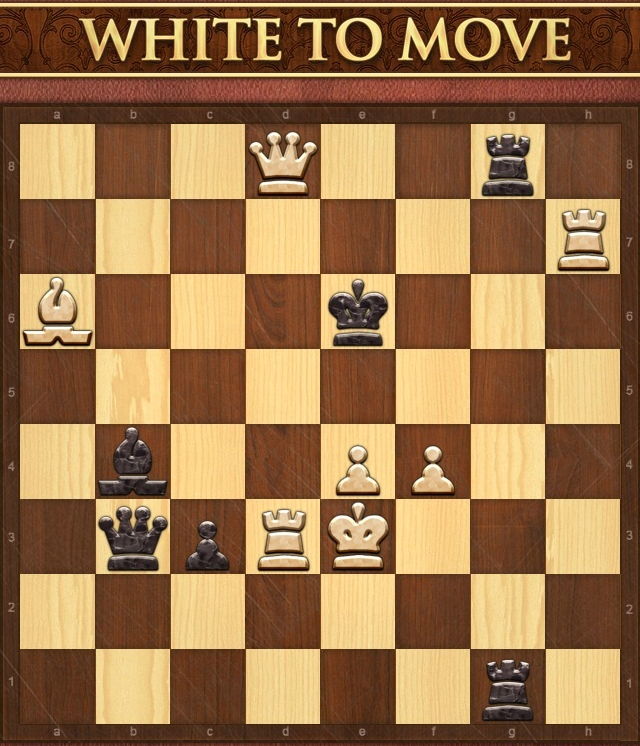
\includegraphics[scale=0.3]{cropped-boards/4-crop.png}} \\
\end{tabular}

\begin{tabular}{cc}
    \num\putindeepbox[7pt]{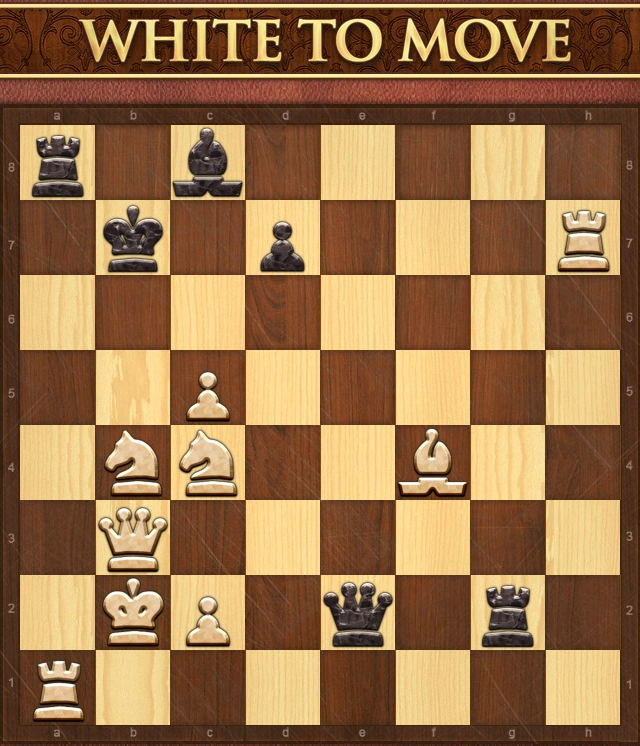
\includegraphics[scale=0.4]{cropped-boards/5-crop.png}}
    & \num\putindeepbox[7pt]{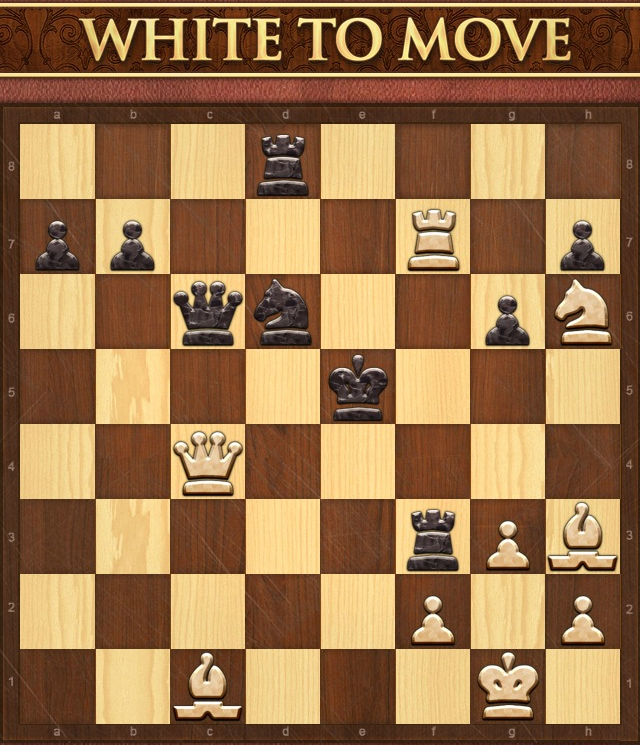
\includegraphics[scale=0.4]{cropped-boards/6-crop.png}} \\
    \num\putindeepbox[7pt]{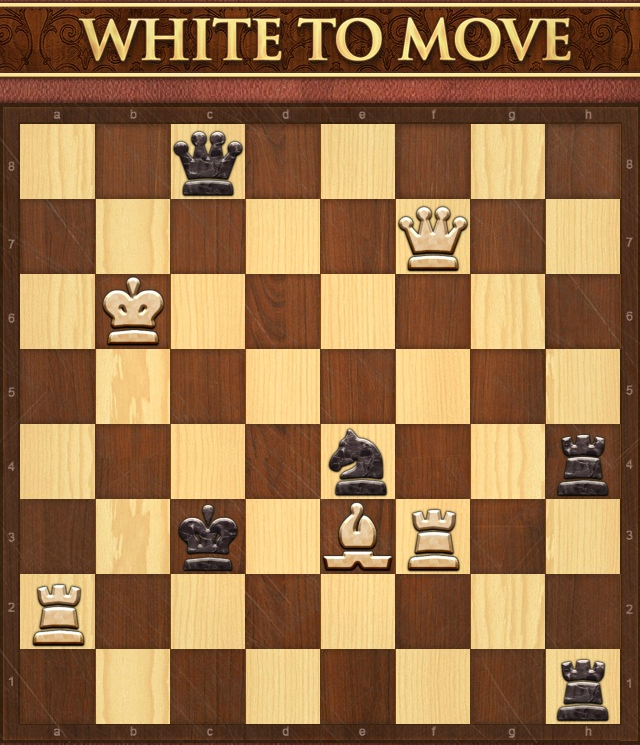
\includegraphics[scale=0.4]{cropped-boards/7-crop.png}}
    & \num\putindeepbox[7pt]{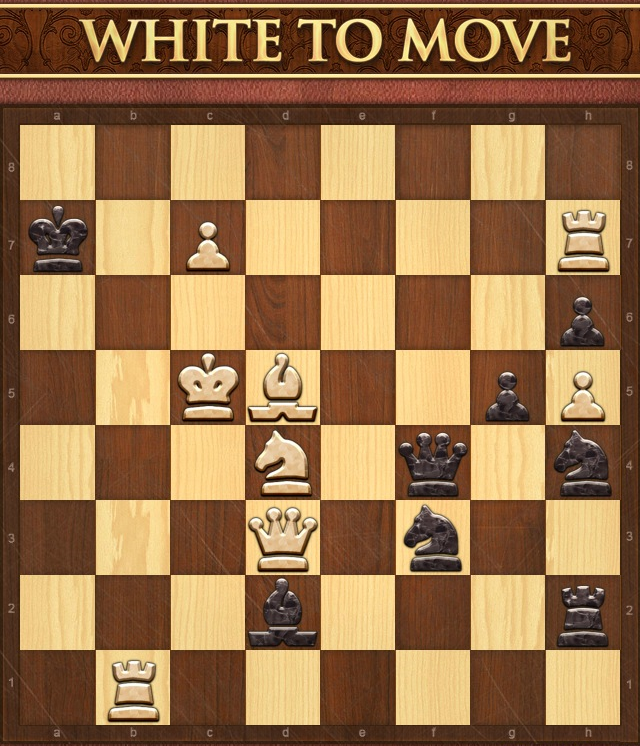
\includegraphics[scale=0.4]{cropped-boards/8-crop.png}} \\
\end{tabular}

\end{document}
